\documentclass[11.5pt]{report}

%------------------- declaring packages---------------------------------


% styling and graphics-based

\usepackage{graphicx} 
\usepackage{emptypage}
\usepackage{geometry}
\usepackage{setspace}
\usepackage{pgf}
\usepackage{pgffor}
\doublespacing

% for figures and tables

% figures:
\usepackage{subfigure}  
\usepackage{adjustbox}
\usepackage{wrapfig}
\usepackage{subfigure}
\usepackage{rotating}
\usepackage{lscape}
% tables:
\usepackage{tabularx,ragged2e,booktabs,caption}
\usepackage{multicol,tabularx,capt-of}
\usepackage{hhline}
\usepackage{multirow}
\usepackage{array}


% for math equations

\usepackage{amssymb}
\usepackage{float}
\usepackage{verbatim}
\usepackage{amsmath} 
\usepackage{amsthm}   
% doble columna 
\usepackage{multicol}

% for acronyms and glossaries

\usepackage{acronym}
\usepackage{glossaries}
%%%%%PRUEBA%%%%

% for hyperlinks
\usepackage{textgreek}


%\usepackage{natbib}
\usepackage[colorlinks = true,
            linkcolor = black,
            urlcolor  = blue,
            citecolor = black,
            anchorcolor = blue]{hyperref}

\usepackage{sectsty}
\allsectionsfont{\bfseries}
\chapterfont{\centering\Large}
\sectionfont{\normalsize}
\subsectionfont{\normalsize}


\usepackage[spanish, mexico]{babel}
\usepackage[autostyle, spanish = mexican]{csquotes}
\MakeOuterQuote{"}


% header formatting

\usepackage{layout}
\usepackage{fancyhdr}
\pagestyle{fancy}
\fancyhf{}
\fancyhead[R]{\thepage}
\fancyhead[L]{\textbf{\nouppercase{\rightmark}}}
\fancyfoot[L]{}

\fancypagestyle{custompagestyle}{%
    \fancyhf{}
    \fancyhead[R]{\thepage}
}

\fancypagestyle{noheaderfooter}{%
    \fancyhf{} % Clear header and footer
    \renewcommand{\headrulewidth}{0pt} % Remove header line
}


%footer formatting

\interfootnotelinepenalty=10000 

\usepackage{epstopdf}
%usas las citas con titulo 
%\usepackage[articletitle=true]{achemso}
%%%%%%%%%%%% usar las citas pero sin titulo  %%%%%%
\usepackage{achemso} 
%\usepackage{libertine}
%\usepackage[superscript]{cite}
\usepackage[utf8]{inputenc}
\usepackage[T1]{fontenc}
\usepackage{lipsum}
\usepackage[justification=centering]{caption}
\usepackage{fontawesome5}
%----------------------------begin document-------------------------------

\begin{document}
%\frontmatter
    % Establece la numeración en 3 para que la siguiente sea 4

\begin{titlepage}
%    \begin{center}
%            
%       
%
%        \large
%        {Evaluacion de la serie \textit{in house} de compuestos LQM 700's en proteinas de \textit{Flavivirus} como Dengue y Zika  }
%
%        \vspace{1.5cm}
%
%        Por
%            
%        \vspace{1.5cm}
%            
%        \large{\uppercase{Luis Alfonso Cárdenas Granados}}
%            
%        \vspace{1.5cm}
%            
%        \normalsize Trabajo que presenta  \\
%        para obtener el grado  \\
%        de Maestro en Ciencias Químicas
%            
%        \vspace{1.0cm}
%            
%            
%        
%        Universidad Nacional Autonoma de México\\
%        México\\
%        2025
%            
%    \end{center}
\newcommand{\Universidad}{\LARGE\textsc{Universidad Nacional Atónoma de México}} %Mantener la primera letra de cada palabra en mayúscula y lo demás en minúsculas
\newcommand{\Programa}{PROGRAMA DE MAESTRÍA Y DOCTORADO EN CIENCIAS QUÍMICAS}
\newcommand{\Campus}{FACULTAD DE ESTUDIOS SUPERIORES CUAUTITLÁN}%Mantener la primera letra de cada palabra en mayúscula y lo demás en minúsculas
\newcommand{\Titulo}{\textsc{Búsqueda de Moléculas con Actividad en Proteínas
	Encargadas de la Replicación Viral para el Virus del Dengue y Zika por Medio de \\ Técnicas \textit{In Silico}}}
\newcommand{\Grado}{MAESTRO EN CIENCIAS}
\newcommand{\Autor}{LUIS ALFONSO CÁRDENAS GRANADOS}
\newcommand{\Asesor}{DR. ENRIQUE ÁNGELES ANGUIANO}
\newcommand{\LugarDeTrabajo}{CUAUTITLÁN IZCALLI, ESTADO DE MÉXICO}
\newcommand{\Fecha}{2025}
\newgeometry{left=2cm,right=2cm,top=2cm,bottom=2cm}
\thispagestyle{empty} % no numeramos la pagina
\pagenumbering{Roman}
%%%%%%%%%%%%%%%%%%%%%%%%%%%% Portada %%%%%%%%%%%%%%%%%%%%%%%%%%%%%%%%%%%%%

\begin{center} %Primera portada
	\centering{
\includegraphics[width=3.25cm]{Figure/UNAMLOGO}}
	
	\LARGE \textbf{\Universidad}\\[0.5cm]
	
	\large \textbf{\Programa}\\ [0.7cm]
	\textsc{\Titulo}\\[1cm]
	\large \textbf{TESIS}
	
	PARA OPTAR POR EL GRADO DE\\ [0.5cm]
	
	\Large\textbf{\Grado}\\ [1cm]
	
	
	\large PRESENTA\\ 
    \Autor\\ [1cm]
	
	\large \Asesor\\
	\Campus\\ [2cm]
	
	CIUDAD UNIVERSITARIA, SEPTIEMBRE 2025.
	
\end{center}
\newpage
\thispagestyle{empty}
\begin{center} %Segunda portada
	\vspace*{1cm}
	\centering{
\includegraphics[width=6.86cm]{Figure/PosgradoLOGO}}\\[1cm]
	
	\LARGE \textbf{\Universidad}\\[0.5cm]
	
	\large \textbf{\Programa}\\ [1cm]
	
	
	\textsc{\textbf{\Titulo}}\\[1.5cm]
	
	
	\large \textbf{TESIS}
	
	\textbf{PARA OPTAR POR EL GRADO DE}\\ [0.5cm]
	
	\Large\textbf{\Grado}\\ [0.5cm]
	
	
	\large \textbf{PRESENTA}\\ 
	\textbf{	\Autor}\\ [1cm]
	
	
\includegraphics[width=6.88cm]{Figure/PosgradoLOGO2}\hspace*{1cm}Ciudad de México, 2025.
	
\end{center}
\restoregeometry
\end{titlepage}
\newpage
\pagestyle{empty}
\newgeometry{left=2cm,right=2cm,top=2cm,bottom=2cm}
\begin{center}
	\textbf{\Large\textsc{Jurado Asignado}}\\[1.5cm]
	
	
\begin{tabular}{p{3.5cm}l}
	\textbf{Presidente}	& Fausto Colón\\ 
	\textbf{Vocal} & Ubaldo Díaz\\
	\textbf{Vocal} & Cipriano Pulido\\
	\textbf{Vocal} & Apolinario Cifuentes\\
	\textbf{Secretario}& Ciriaco Ríos\\
\end{tabular}\\[1.5cm]

	\textbf{\textsc{Lugar Donde se Realizó la Tesis}}\\[.6cm]
	
	Esta tesis se realizó en el \ac{LQM} de la Facultad de Estudios Superiores Cuautitlán y en el Laboratorio 111 del conjunto E de la Facultad de Química.\\[1.5cm] 
	
	\textbf{CONGRESOS}\\[0.6cm]
	
	Durante el periodo de maestría se asistió al congreso-taller \textbf{UGM \& Conference 2024} del 25 al 28 de Junio del 2024 en Montreal, Canadá organizada por \ac{MOE} y se presentaron parte de los resultados obtenidos en esta tesis en un póster con titulo: "Investigating Compounds for Flavivirus E Protein Inhibition: Implication for DENV and ZIKV".\\[1.5CM]	
	\textbf{\textsc{Participación en Artículos no Derivados de esta Tesis Durante la Estancia de Maestría }}\\[0.6cm]
	\begin{itemize}
		\item Hernández-Serda MA, Vázquez-Valadez VH, Aguirre-Vidal P, Markarian NM, Medina-Franco JL, \textbf{Cardenas-Granados LA}, Alarcón-López AY, Martínez-Soriano PA, Velázquez-Sánchez AM, Falfán-Valencia RE, Angeles E, Abrahamyan L. \textbf{\textit{In Silico} Identification of Potential Inhibitors of SARS-CoV-2 Main Protease (Mpro).} Pathogens. 2024 Oct 11;13(10):887. doi: 10.3390/pathogens13100887. PMID: 39452758; PMCID: PMC11510711.
		\item Hernández-Serda MA, Alarcón-López AY, Vázquez-Valadez VH, Briseño-Lugo P, Martínez-Soriano PA, Leguízamo V, Torres N, González-Terán R, \textbf{Cárdenas-Granados LA}, Sánchez Muñoz F, Rodríguez E, Lerma C, Zúñiga Muñoz AM, Ángeles E, Carbó R. \textbf{Hypoxic Cardioprotection by New Antihypertensive Compounds in High Salt-Diet Hypertensive Rats: Glucose Transport Participation and Its Possible Pathway.} Int J Mol Sci. 2024 Aug 13;25(16):8812. doi: 10.3390/ijms25168812. PMID: 39201496; PMCID: PMC11354541.
		\item Alarcón-López, A., Hernández-Serda, M., Aguirre-Vidal, P., \textbf{Cárdenas-Granados, L.}, Vázquez-Valadez, V., Martínez‑Soriano, P., Briseño-Lugo, P., Velázquez-Sánchez, A., Rul-Ramírez, E., Jiménez-Jiménez, M. L., Becerril-Ricco, J., De Guevara, A. A., Tinajero-Rodríguez, J. M., Ortiz, E., \& Ángeles, E. (2023). \textbf{Computational insight and anticancer effect of cinnamic Acid-Derivative amide compounds.} Journal of the Brazilian Chemical Society. https://doi.org/10.21577/0103-5053.20230195.
		\item Alarcón-López, Y. A., Aguirre-Vidal, P., Vásquez-Valadez, H. V., Hernández-Serda, A. M., \textbf{Cárdenas-Granados, A. L.}, De La Garza, C. E. E., Pérez, N. O., Angeles, E., \& Martínez, V. P. M. (2025).\textbf{ \textit{In silico} and experimental evidence for the stabilization of RHEPO by glycine, glutamic acid and lysine.} AAPS PharmSciTech, 26(1). https://doi.org/10.1208/s12249-024-03008-0
		
	\end{itemize}
%	\lipsum[2-2]
	
\end{center}
\restoregeometry


\pagenumbering{roman}  % Usa números romanos para las páginas preliminares
\setcounter{page}{3}
\chapter*{Dedicatoria}\

Para alguien

\addcontentsline{toc}{chapter}{Dedicatoria}

\chapter*{Abstract}

El dengue chinga mucho, especialmente al que hace la tesis $\beta$-OG \ac{LQM}

\addcontentsline{toc}{chapter}{Abstract}

\chapter*{Agradecimientos}

A Gronda triple x ANDELE
\lipsum
\addcontentsline{toc}{chapter}{Agradecimientos}

\tableofcontents{}

\cleardoublepage
\addcontentsline{toc}{chapter}{Indice de tablas}
\listoftables{}

\cleardoublepage
\addcontentsline{toc}{chapter}{Indice de figuras}
\listoffigures{}

\cleardoublepage
\addcontentsline{toc}{chapter}{Abreviaturas}
\chapter*{ABREVIATURAS}
%\thispagestyle{noheaderfooter}

\begin{multicols}{2}
\begin{acronym}
% list down all your acros here
{\fontsize{10}{9}\selectfont
\acro{ADN}{Ácido Desoxiribonucleico}
\acro{ARN}{Ácido Ribonucleico}
\acro{DENV}{Virus del Dengue}
\acro{ZIKV}{Virus del Zika}
\acro{PDB}{\textit{"Protein Data Bank"}}
\acro{VMD}{\textit{"Visual Molecular Dynamics"}}
\acro{GNM}{\textit{"Gaussian Normal Modes"}}
\acro{NMA}{\textit{"Normal Modes Analysis"}}
\acro{NOG}{\textit{"N-Octyl-Glucoside"}}
\acro{MOE}{Molecular Operating Enviroment}
\acro{LQM}{Laboratorio de Química Medicinal }
\acro{POPC}{POPC}
\acro{ICTV}{\textit{"International Committee on Taxonomy of Viruses"}}
\acro{CZS}{Congenital Zika Syndrome}
\acro{NTD}{Neglected Tropical Diseases}
\acro{CAPE}{\textit{"Caffeic Acid Phenyl Ester"}}
\acro{RMSD}{\textit{"Root Mean Square Deviation"}}
\acro{RMSF}{\textit{"Root Mean Square Fluctuation"}}
\acro{BOG}{$\beta$-OG site}
\acro{ADMET}{\textit{"Absortion Distribution Metabolism Excretion Toxicity"}}
\acro{RdRp}{\textit{"RNA-dependent RNA polymerase"}}
\acro{YFV}{Virus de la Fiebre Amarilla}
\acro{WNV}{Virus del Nilo Occidental}
\acro{E}{Proteína de Envoltura}
\acro{C}{Cápside}
\acro{prM}{Proteína de Pre-Membrana}
\acro{M}{Proteína de Membrana}
\acro{pr}{Proteína pr}
\acro{M}{Proteína de Membrana}
\acro{JEV}{Virus de Encefalitis Japonesa}
\acro{NS}{Proteína no estructural}
\acro{ORF}{\textit{"Open Reading Frame"}}
\acro{RE}{Retículo Endóplasmático}
%\acro{RdRp}{ARN polimerasa dependiente de ARN}
}
\end{acronym}
\end{multicols}





\thispagestyle{noheaderfooter}

\pagenumbering{arabic}


%Antecedentes%
\chapter{Antecedentes}
\label{ch1}

\section{Virus}

Los virus así como las bacterias son organismos microscópicos con capacidad infecciosa, a diferencia de las bacterias, los virus necesitan parasitar células del hospedero para apoderarse de su capacidad de síntesis proteica, los virus pueden afectar a diversos organismos, desde animales, bacterias, plantas hasta hongos. \cite{Racaniello2020}

La presencia de los virus en nuestra vida y el ambiente es de suma importancia, parte de nuestra información genética al rededor de un 5-8\% tiene origen viral, ademas de esto no todos los virus tienen la capacidad de generar efectos negativos, existen virus que tienen efectos benéficos, como aquellos que se encuentran en el mar y se encargan de parasitar bacterias, siendo parte fundamental de la cadena biológica marina. Por otro lado los virus que presentan un efecto negativo, como es el caso de la reciente pandemia ocasionada por el virus del \textit{SARS-COV2}, estos patógenos  pueden tener efectos muy diversos, diversos en el sentido de las enfermedades que pueden causar, así como los distintos órganos o tejidos que atacan y en tamaños. Desde los picornavirus con un tamaño al rededor de 300 \AA \, o los bacteriófagos entre 70-200 nm llegando hasta el caso de los pandoravirus con un tamaño de 1000 nm. \cite{Racaniello2020,Rossmann2013,Van2022}
\subsection{Partículas Virales}
Las partículas virales en su exterior pueden encontrarse desnudas presentando unicamente una capside que es la asociación de múltiples proteínas con el fin de cubrir el material genético o aquellos virus denominados virus con envoltura, dicha envoltura de origen membranoso, está formada por lípidos pertenecientes a la célula del hospedero. En su mayoría los virus que afectan humanos poseen una forma esférica y presentan una variedad de proteínas y material genético. Este arreglo macromolecular tan diverso da forma a lo que se conoce como virión, el cual tiene distintos propósitos como la protección del frágil material genético y fungir como vehículo para continuar con el ciclo de replicación. \cite{Racaniello2020,Van2022}

Como lo muestra la figura \ref{Tipos_virus} sobre los virus con envoltura y sin envoltura residen proteínas conocidas como glucoproteínas, las cuales son proteínas unidad a azucares por medio de enlaces covalentes, de donde existen dos tipos de glucosilaciones principales, las N-Glucosilaciones y las O-Glucosilaciones, las primeras unidas a un residuo de Asparagina (N) y las ultimas normalmente unidas a un residuo de Serina (S) o Treonina (T), generalmente las glucoproteínas presentes en la superficie del virión tienen una función de adhesión a un receptor o un co-receptor que facilite la entrada del virión a la célula.\cite{Racaniello2020,Van2022,Idris2016}
\begin{figure}[H]
    \centering
    
\includegraphics[width=3.0in, height=3.0in]{Figure/latex_fig_1.png}
    \caption{putos...}
    \label{Tipos_virus}
\end{figure}

\subsection{Clasificación de Baltimore}
Debido a la gran variedad de virus, debe existir una forma de clasificarlos, existe la  forma taxonómica de la cual se comentara posteriormente, por otro lado existe una forma de clasificación viral basada en el material genético encapsulado dentro del virus, propuesta originalmente en 1971 por David Baltimore donde se enfocaba en el genoma de distintos virus ya sean de \ac{ADN} o \ac{ARN} y originalmente propuso 6 grupos a los cuales después de varios años se añadió un grupo extra, los cuales en conjunto son conocidos como las 7 clasificaciones de Baltimore, la importancia de esta clasificación es debido a que permite seguir la ruta de la información genetica de los virus hasta el momento de la síntesis de sus proteínas, mostrando como todos los virus son entes que se apoderan de el mecanismo de producción de ARN mensajero.\cite{Baltimore1971, Racaniello2020}\cite{Koonin2021}
	\begin{itemize}
	\item Clasificación I: Se trata de virus de \ac{ADN} de doble cadena.
	\item Clasificación II: Son virus de cadena sencilla de \ac{ADN}.
	\item Clasificación III: Aquellos virus de \ac{ARN} de doble cadena.
	\item Clasificación IV: Son virus de \ac{ARN} de cadena sencilla en sentido positivo.
	\item Clasificación V: Virus de \ac{ARN} de cadena sencilla en sentido negativo.
	\item Clasificación VI: Virus de \ac{ARN} en sentido positivo de transcripción inversa.
	\item Clasificación VII: Virus de doble cadena de \ac{ADN} con segmentos incompletos.
	\end{itemize}

En la figura \ref{BaltimoreClass} A se esquematiza el flujo de información desde que el material se encuentra dentro del virión hasta la formación de \ac{ARN} mensajero, de acuerdo a sus características algunos virus podrían caer dentro de dos categorías, o el reciente descubrimiento de virus de \ac{ARN} de ambisentido, que contiene dos o tres segmentos, generando problemas con esta clasificación. \cite{Koonin2021}

\subsection{Clasificación Taxonómica}
Establecida en 1975 como el \ac{ICTV} se encarga de la clasificación y nomenclatura taxonómica de los distintos virus, ácidos nucleicos satélites, viriformes y viroides, conformado por una variedad de virólogos, sirviendo como punto de referencia para la taxonomía viral (https://ictv.global),actualmente hasta la ultima revisión de 2024 se encuentran 368 familias y 16,215 especies, aunque existen otras clasificaciones no basadas en taxonomía, como pueden ser la clasificación de Baltimore o aquellas basadas en características fenotípicas, solo existe una clasificación taxonómica aprobada, y es aquella emitida por el \ac{ICTV} que esta basada plenamente en relaciones evolucionarias, donde se deben de tratar de grupos monofiléticos basados en relaciones evolucionarias. \cite{Siddell2023}
 
La imagen \ref{BaltimoreClass} B muestra la unión entre la clasificación de Baltimore y la taxonómica, donde las lineas mas gruesas representan una mayor asociación, se observa que en la mayoría de las clasificaciones de Baltimore se comparten un ancestro común con el reino \textit{Riboviria}.\cite{Koonin2021}


\begin{figure}[H]
	\centering
	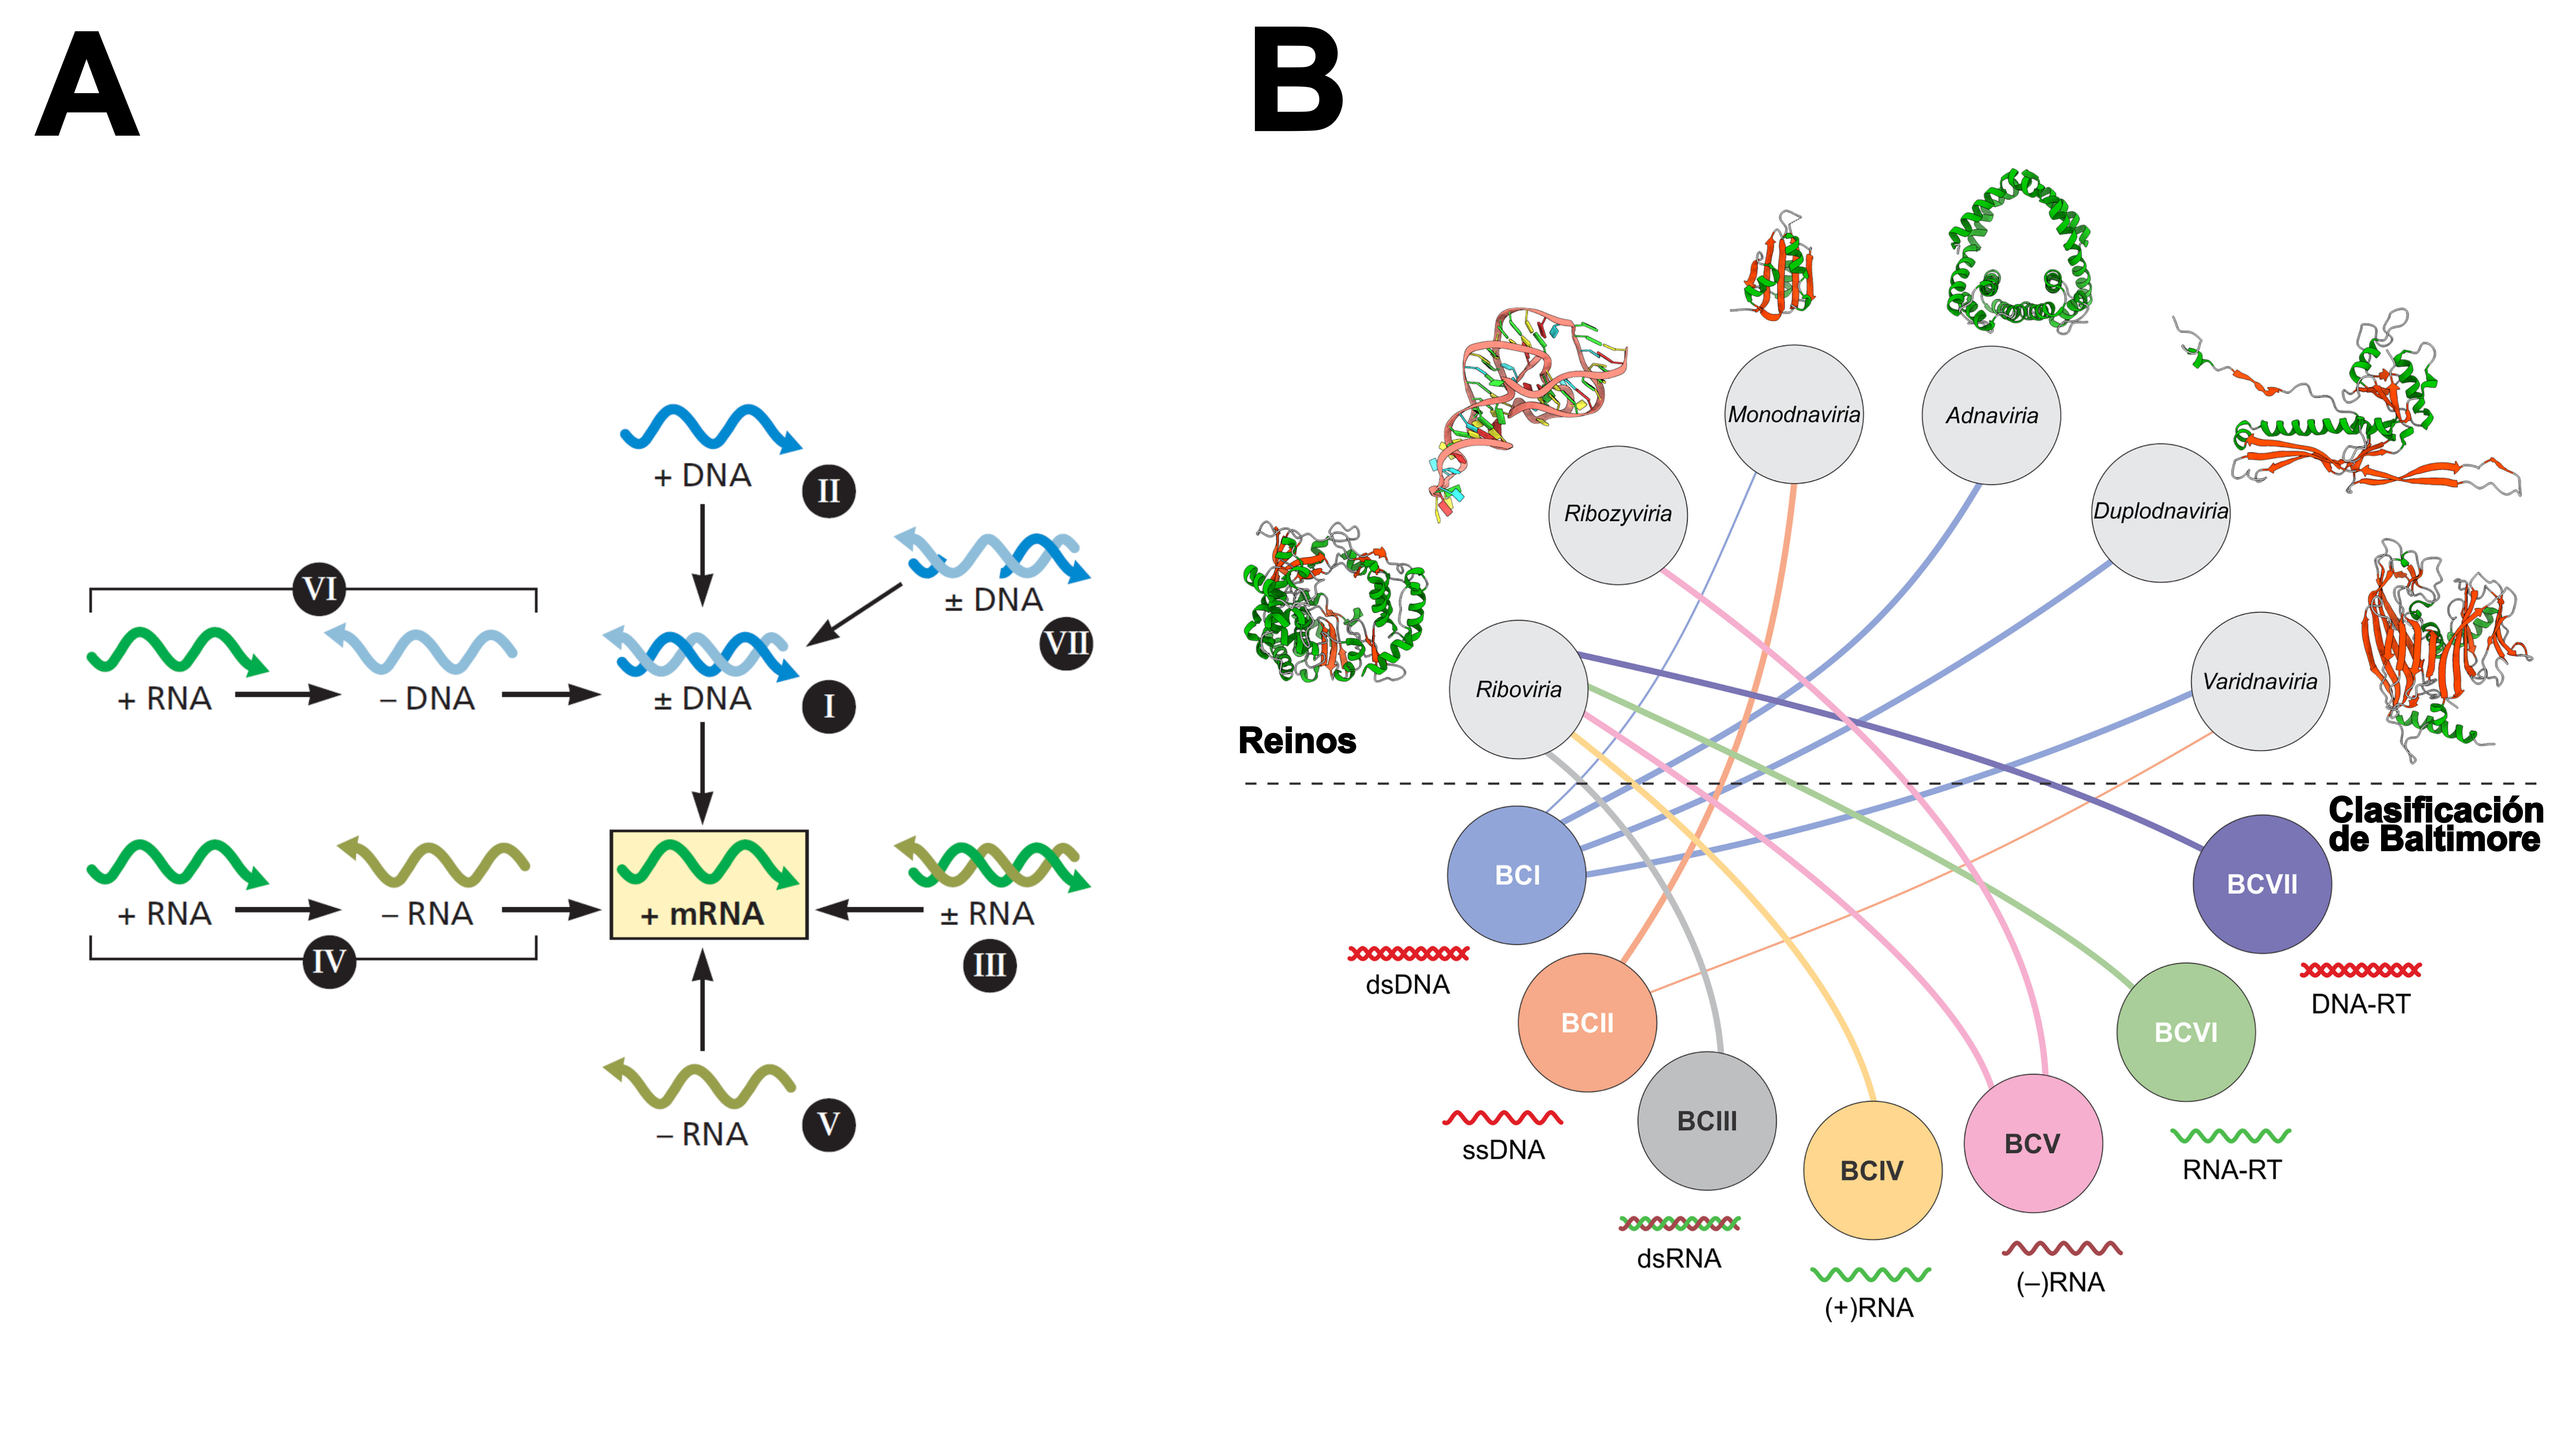
\includegraphics[width=\textwidth]{Figure/BaltimoreClass.png}
	\caption[Clasificación de Baltimore]{A) Clasificaciones propuestas por Baltimore. B) Visualización de la clasificación de Baltimore en unión con la clasificación Taxonómica (Imagenes modificadas)}
	\label{BaltimoreClass}
\end{figure}
   

\section{Flavivirus}
La familia \textit{Flaviviridae} comprende cuatro géneros: \textit{Hepacivirus}, \textit{Orthoflavivirus}, \textit{Pegivirus} y \textit{Pestivirus}, que incluyen un total de 97 especies. Varios de estos virus son patógenos para los humanos, como el \textit{Orthoflavivirus nilense} (anteriormente conocido como \ac{WNV}), el \ac{YFV}, el \ac{JEV}, el \ac{DENV} y el \ac{ZIKV}. Donde principalmente se ha buscado como estrategia para combatirlas el uso de vacunas, las cuales han funcionado de forma profiláctica en algunos virus como \ac{YFV} y \ac{JEV}. Por lo que para el resto las estrategias se han limitado a la prevención, es decir evitar el contacto con los vectores principales, los cuales son los mosquitos.\cite{VanLeur2021} 

Se trata de virus de ARN de cadena sencilla en sentido positivo, con una longitud de aproximadamente 11 kb. Su genoma presenta un capuchón tipo 1 en el extremo 5' y carece de una cola poli-A en el extremo 3'. Alrededor de las regiones codificantes de proteínas, se encuentran dos áreas no traducidas: una de aproximadamente 100 nucleótidos en el extremo 5' y otra de 400-700 nucleótidos en el extremo 3'. Estos virus están envueltos en una membrana bilipídica derivada de las células del hospedador, y su virión tiene un diámetro aproximado de 50 nm. El material genético de 1 \ac{ORF} codifica una única proteína que, posteriormente, es escindida por diferentes proteasas del virus o del hospedador como lo muestra la figura \ref{Poliprot}. Tres de estas proteínas son estructurales (\ac{C}, \ac{E} y \ac{prM}), mientras que siete son de carácter \ac{NS} (NS1, NS2A, NS2B, NS3, NS4A, NS4B, NS5). La cápside está cubierta por una membrana derivada del hospedador, y en su superficie exterior se encuentran 90 homodímeros de las proteínas \ac{E} y \ac{M}, ensambladas en una simetría icosaédrica.\cite{Barrows2018,VanLeur2021}

\begin{figure}[H]
	\centering
	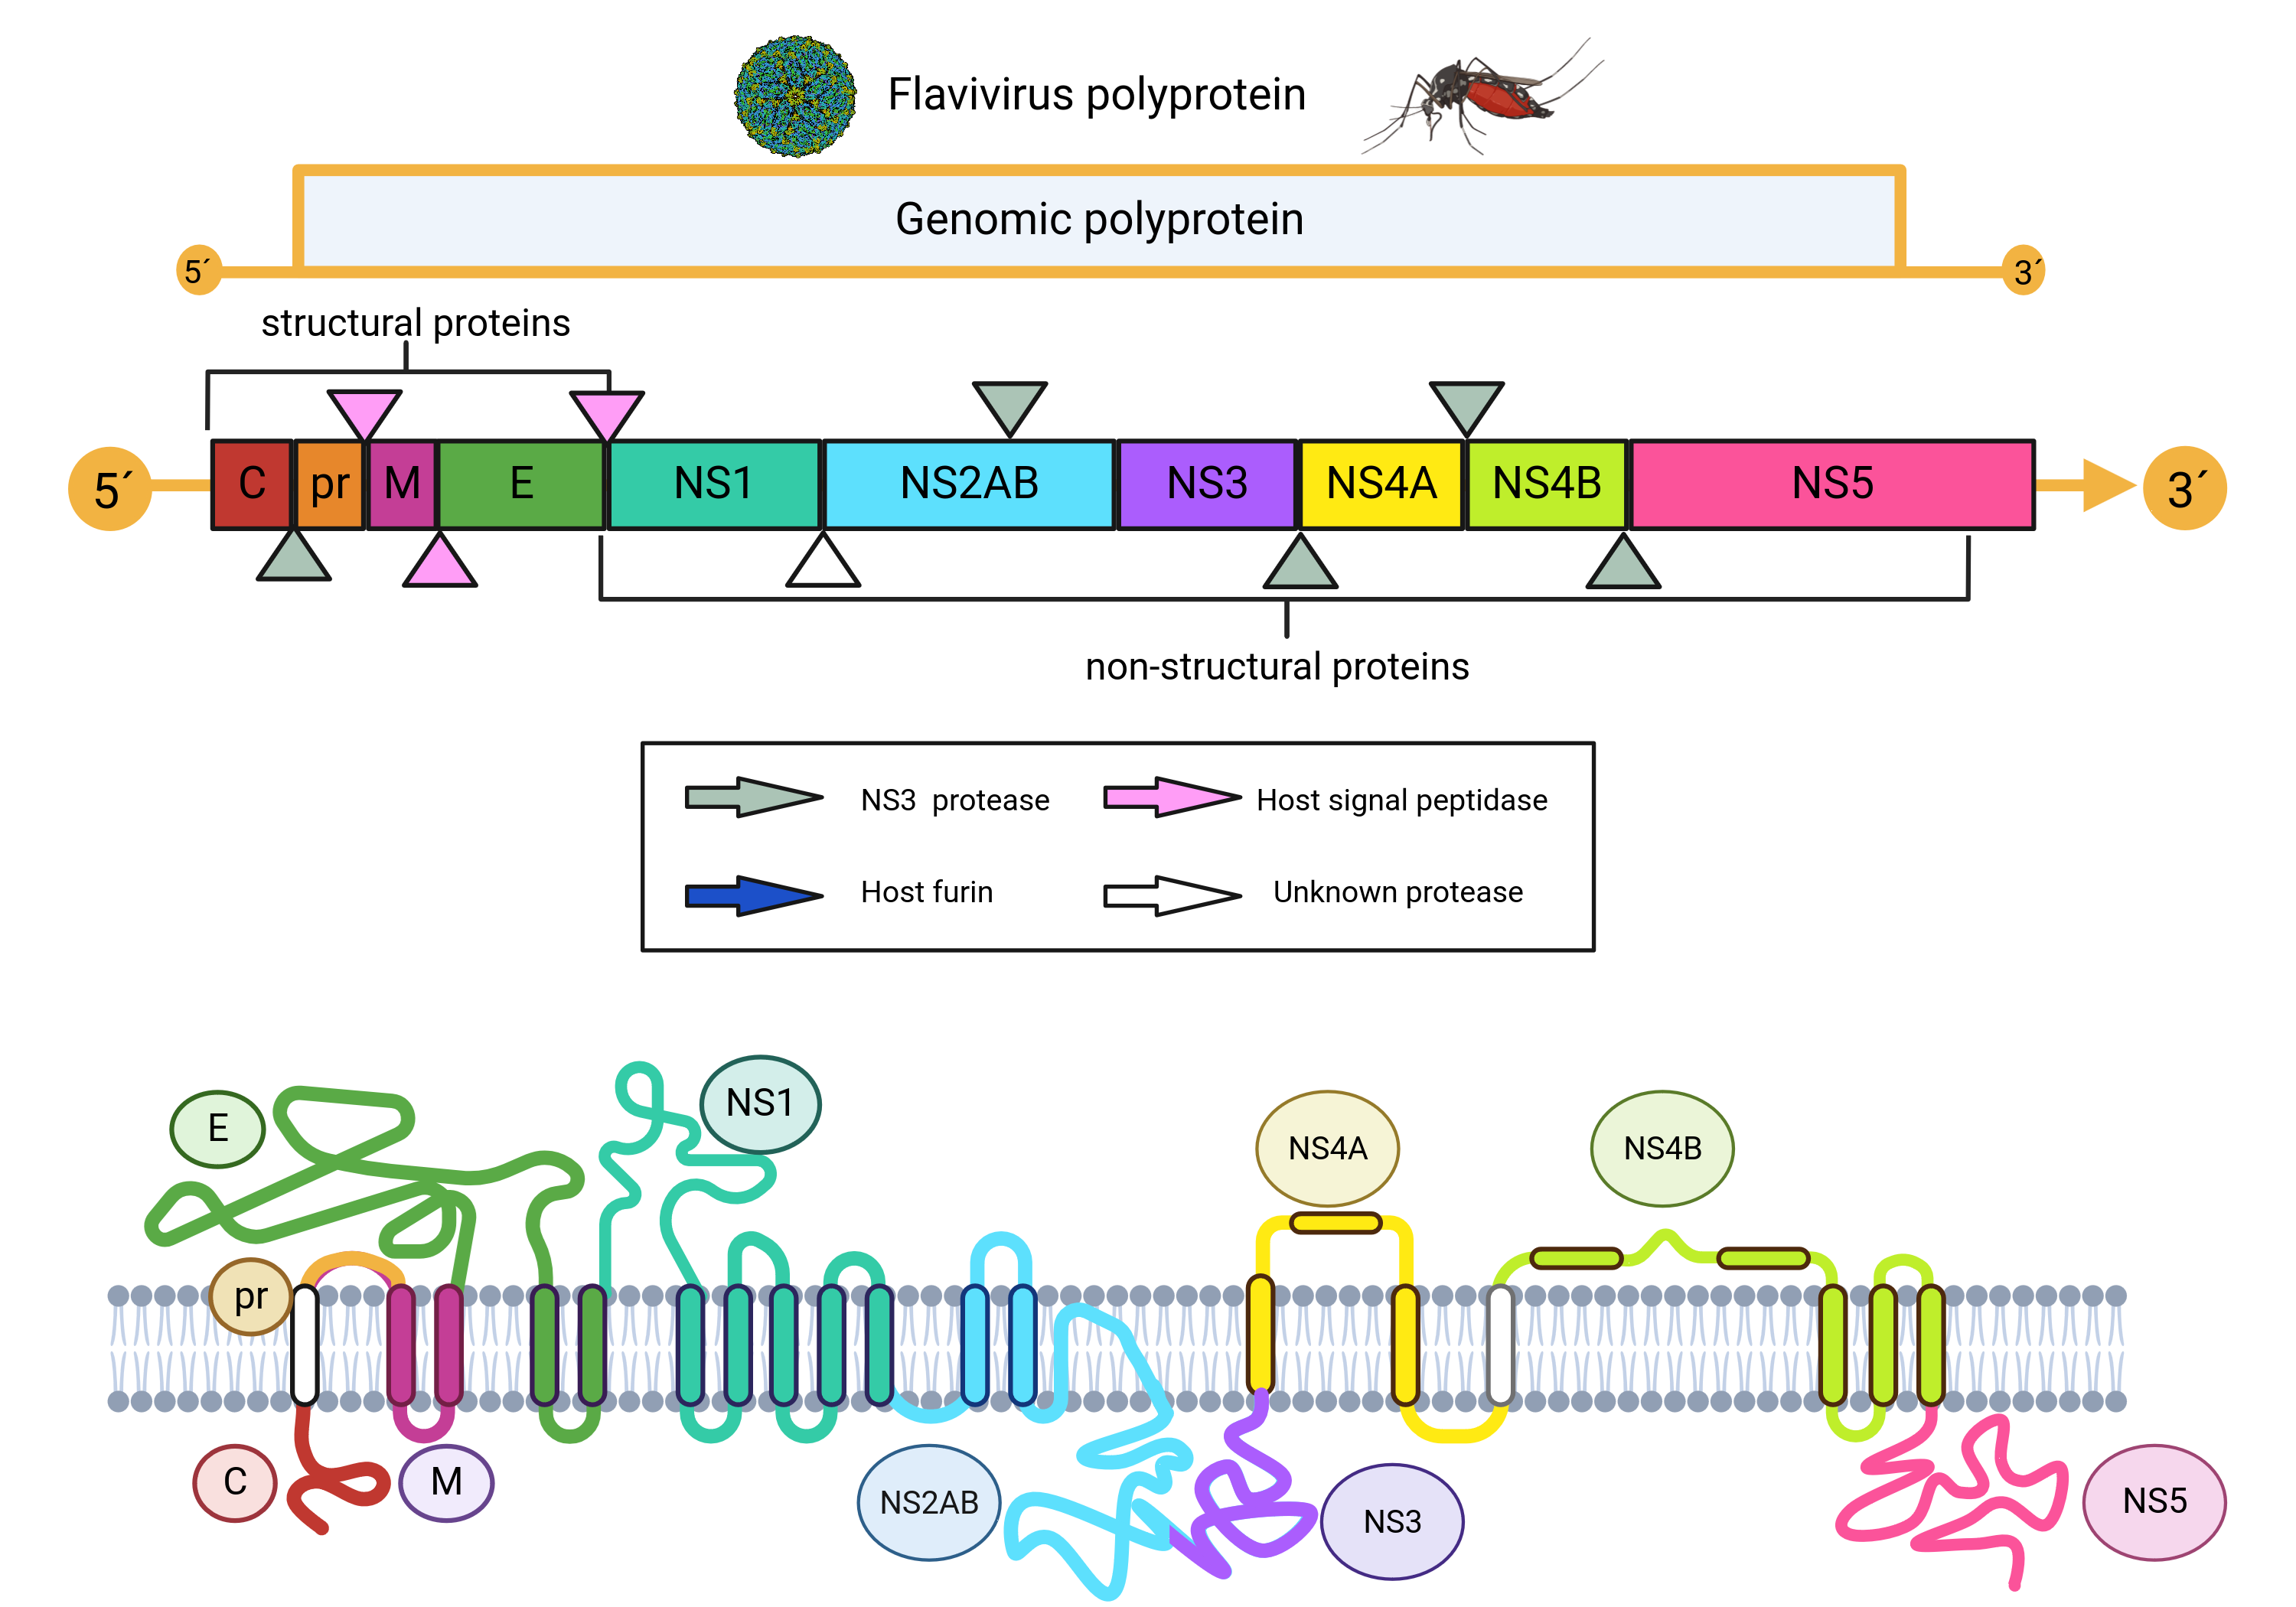
\includegraphics[width=\textwidth]{Figure/03_Polyproteina}
	\caption{Organización general de las proteínas en los Flavivirus}
	\label{Poliprot}
\end{figure}
La proteína \ac{C} es el componente principal al interior de la membrana, con varias copias, se trata de una proteína básica con carga asimétrica de 12kDa donde la región con mayor polaridad interacciona con el material genético mientras que la región apolar lo hace con la membrana. Aunque conserva su estructura y función entre las distintas especies, es de las proteínas con mayor variabilidad genética. Cada monómero contiene al rededor de 3 a 4 hélices alfa, en conjunto con el \ac{ARN} viral forma la nucleocápside de un tamaño aproximado de 30nm.  \cite{Sotcheff2020, VanLeur2021} 

La proteína \ac{prM} durante el ensamblaje del virus se encuentra como una sola proteína con regiones transmembranales y dominios que cubren a la proteína \ac{E} de una fusión prematura, durante la formación del virión la proteína \ac{prM} se asocia con la proteína \ac{E} de forma trimérica, durante el proceso de maduración del virus mientras transita el Golgi esta es escindida por la proteína furina del hospedero transformando la proteína \ac{prM} en dos segmentos, la proteína \ac{pr} y \ac{M}, donde en el virión maduro la proteína M se encuentra de forma homodimérica consigo misma y como heterotetrámero con la proteína \ac{E}, este proceso de maduración resulta ser ineficiente teniendo como consecuencia la presencia de viriones inmaduros o parcialmente maduros, que pueden afectar en el reconocimiento de anticuerpos virales.  \cite{Bernardo-Menezes2022, Majowicz2023,Dowd2014, Mukherjee2016a}

La característica superficie presente en los viriones de los flavivirus se debe a la proteína \ac{E} que se encuentra agrupada debido a las simetría icosaédrica del virus en 30 zonas llamadas "balsas" que están constituidas por 6 unidades de la proteína \ac{E} o 3 homodímeros, la proteína se encuentra dividida en dos regiones; la primera una región de tallo-membrana compuesta principalmente por hélices en el virus maduro y una segunda región llamada dominio ectosoluble esta dividida en tres dominios (DI, DII y DIII), contiene una región altamente hidrofóbica que se conoce como el péptido de fusión, zona de suma importancia en la entrada del virus que sirve como anclaje en la membrana del hospedero, siendo la zona mas conservada entre los distintos flavivirus, por otro lado la proteína \ac{E} responsable del tropismo viral, contiene sitios de glucosilación necesarios en el proceso de adhesión celular así como enlaces disulfuro importantes para el plegamiento de los distintos dominios, en el virión maduro se encuentra dispuesto formando 90 \ac{M}/\ac{E} heterotetrámeros, representado en la figura \ref{proteinasflav}A .\cite{Barrows2018,VanLeur2021,Seligman2008, Marzinek2015, Majowicz2023}

Las funciones de las \ac{NS} son muy diversas desde la activación de la ruta NF-$\kappa$B o el inflamasoma y por eso solo se hace un breve resumen de sus funciones. Las proteínas no estructurales  a pesar de no encontrarse como tal presentes en el virion maduro cumplen otros propositos durante la replicación, las \ac{NS} de los \textit{Flavivirus} son en su mayoría proteasas, como lo muestra la figura \ref{Poliprot} algunas proteínas sirven como proteasas de la poliproteína, principalmente la proteína \ac{NS}2B/\ac{NS}3 y algunas otras proteínas celulares como el caso de la Furina. 

La proteína \ac{NS}1 es abundante en el suero de pacientes infectados, es multifuncional se puede encontrar como monómero en el \ac{RE} en la replicación o como oligómero en otras etapas de la infección y se ha propuesto como proteína diana para combatir la infección por Zika .\cite{VanLeur2021,Latanova2022,Raza2020, Rastogi2016}
  
La proteína \ac{NS}2 se encuentra dividida en dos subproteínas, la \ac{NS}2A de 22-25 kDa de característica transmembranales se propone que tiene funciones importantes en la síntesis de \ac{ARN} así como ayudante para la formación del complejo de replicación y la \ac{NS}2B una proteína integral de membrana, de 14kDa con una región hidrofílica necesaria para la activación de la proteína \ac{NS}3.

La proteína \ac{NS}3 de mayor tamaño que las anteriores de 69 kDa tiene dos dominios, siendo el dominio N-terminal una proteasa similar a tripsina con la capacidad de escindir de forma \textit{cis} o \textit{trans} la poliproteína viral donde es necesaria la presencia de la proteína \ac{NS}2B como cofactor y por otro lado el dominio C-terminal la capacidad de actuar como una helicasa .\cite{Latanova2022}

La proteína \ac{NS}4 al igual que la proteína \ac{NS}2 se divide en dos después de ser escindida, dejando un péptido conocido como 2k insertado en la membrana del \ac{RE}, por su parte la función dela proteína \ac{NS}4A aunque forma parte del complejo de replicación viral, su función completa no esta totalmente entendida.\cite{Barzon2016} La proteína \ac{NS}4B de 27 kDa en su forma madura, presenta dominios transmembranales y participa en el ensamblado del complejo de replicación, tiene interacciones con las \ac{NS} 1,3 y 4A.\cite{Latanova2022,VanLeur2021}

Por otra parte la \ac{NS}5 es la proteína mas conservada entre los \textit{flavivirus}, ademas de ser la mas grande con 105 kDa, su dominio N-terminal tiene funciones de metiltransferasa mientras que la región C-terminal presenta un dominio \ac{RdRp} con funciones de importancia en la replicación del genoma, donde el complejo \ac{NS}3 y \ac{NS}5 presume ser el responsable de la replicasa viral.\cite{Kapoor1995,Latanova2022}




\begin{figure}[h]
	\centering
	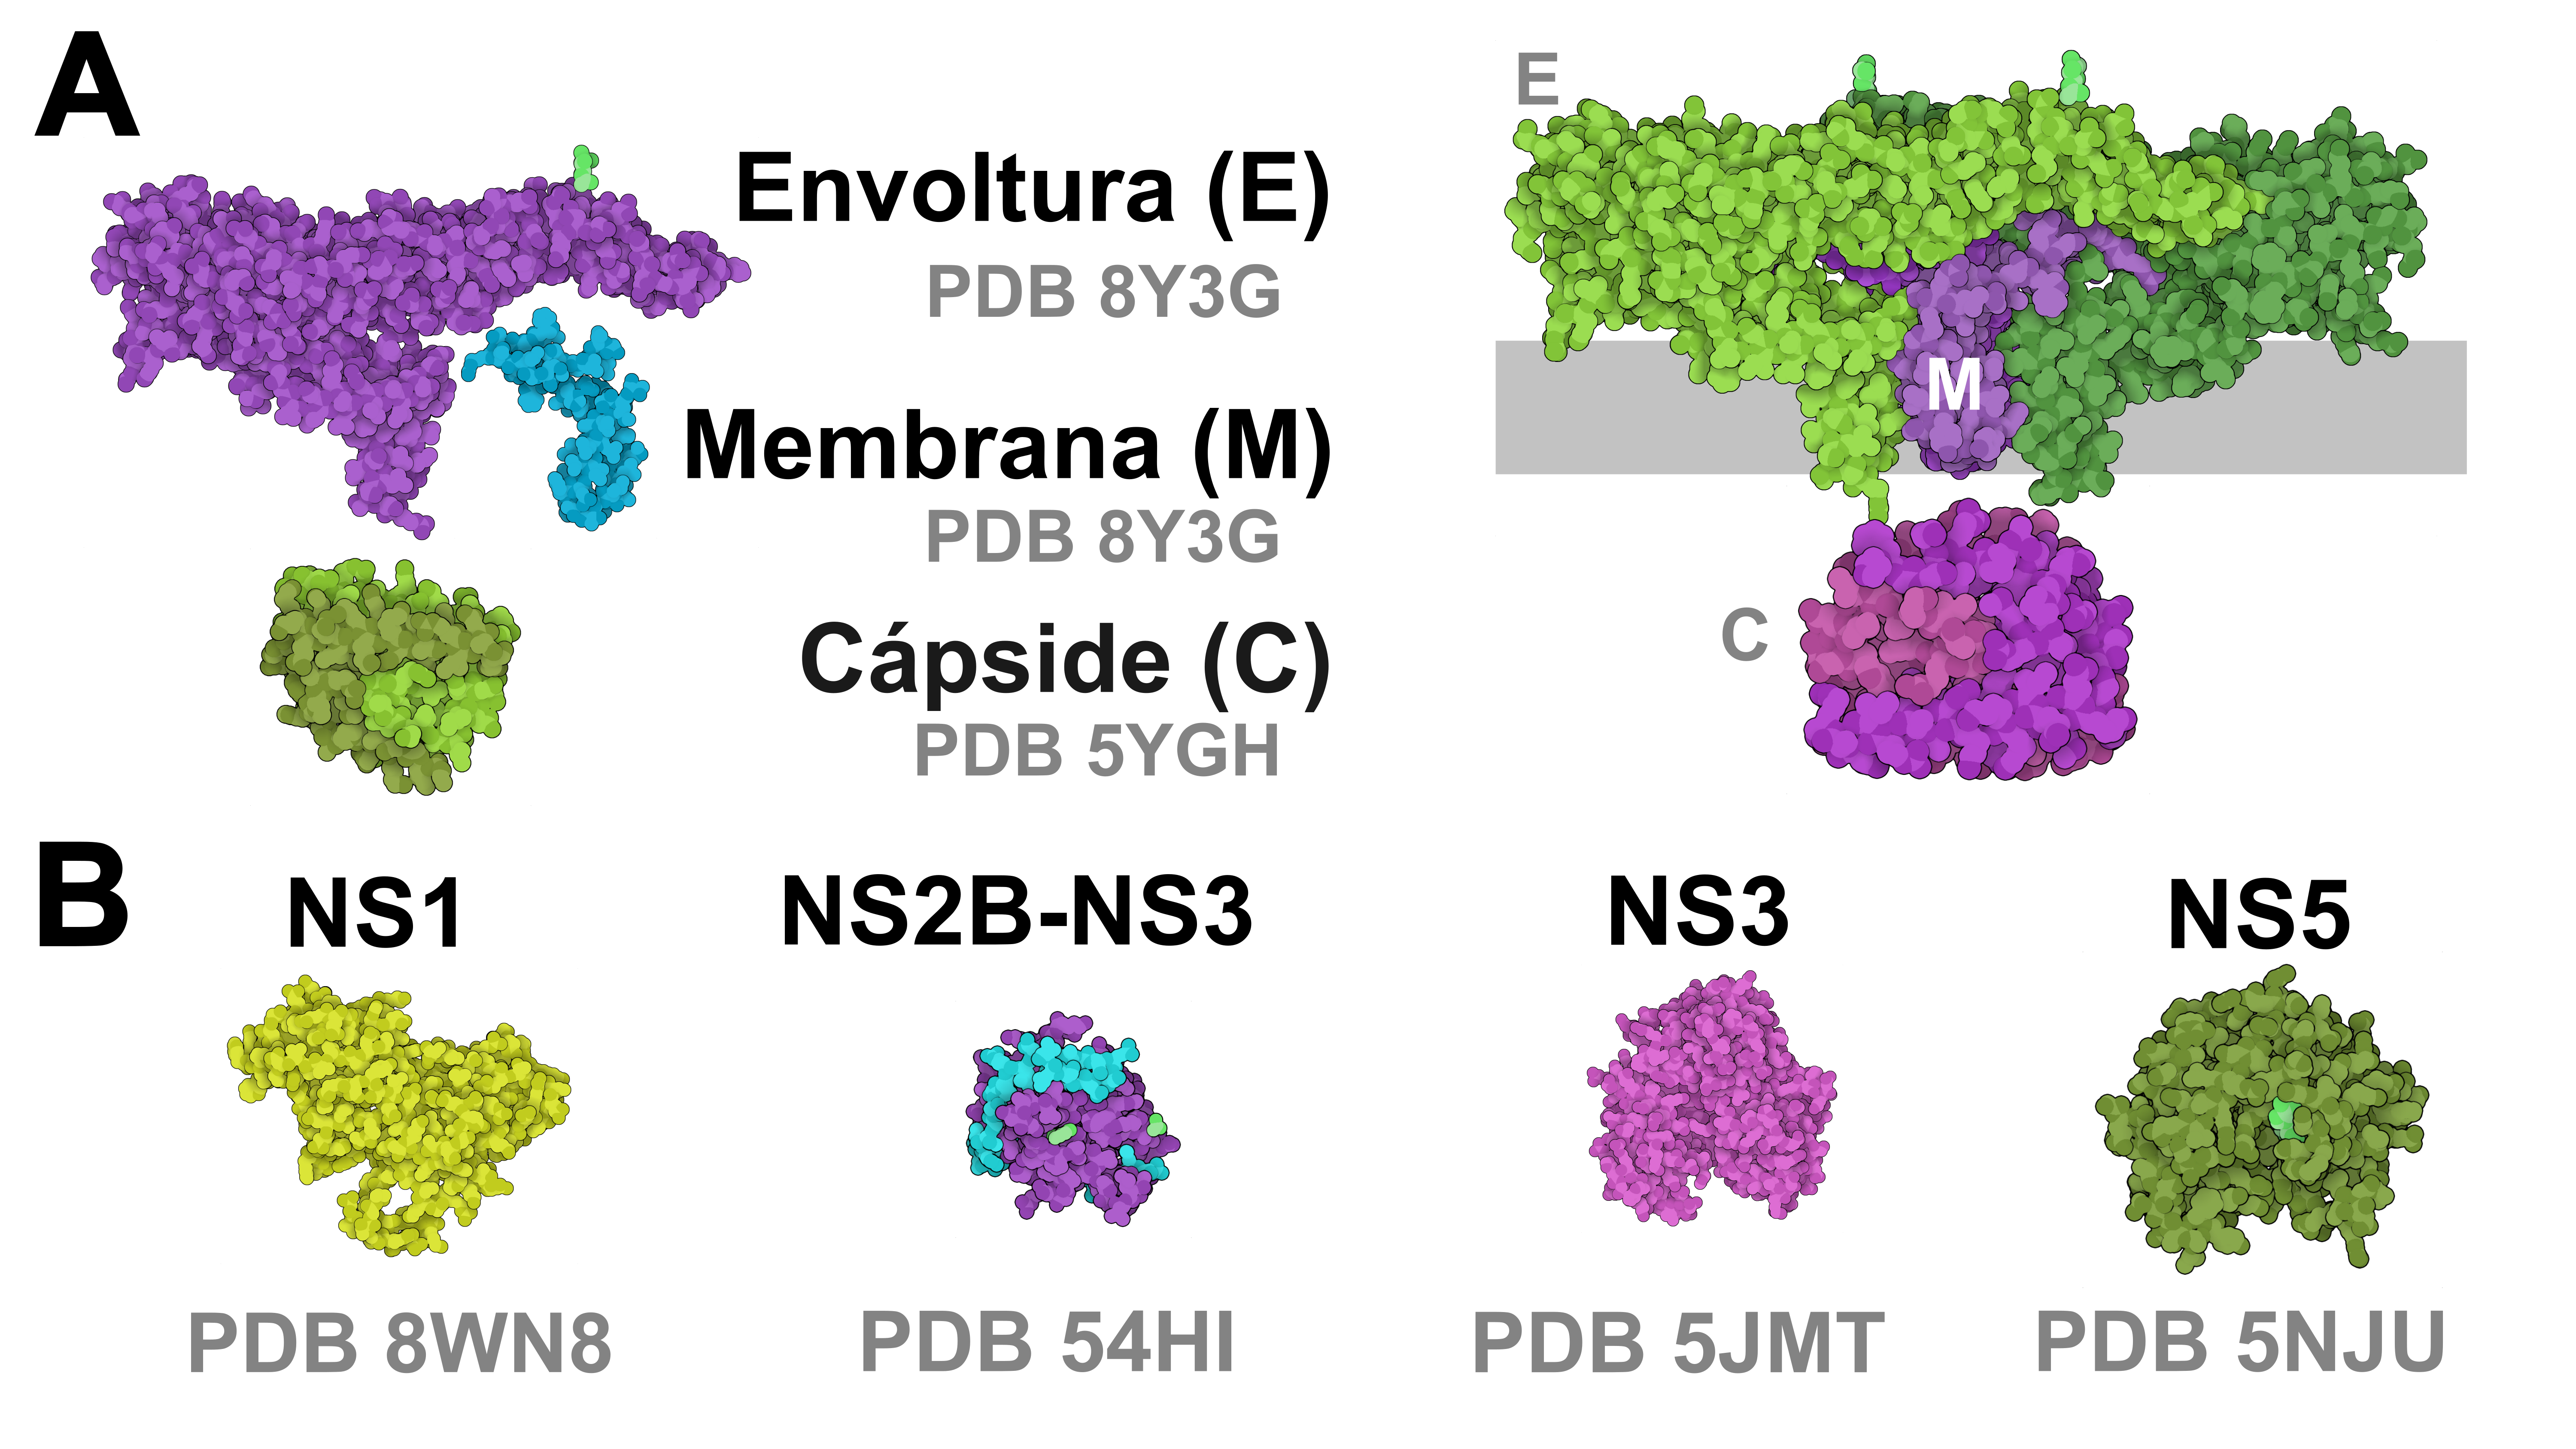
\includegraphics[width=\textwidth]{Figure/Proteinas_flav}
	\caption{A)Proteínas estructurales y modelo de ensamble del complejo C-M-E. B)Proteínas no estructurales}
	\label{proteinasflav}
\end{figure}

\subsection{Ciclo de replicación}

El tamaño y forma de los virus tiene implicaciones en su ciclo de replicación, 
\subsection{Enfermedades Transmitidas por Vectores}
Se le considera vectores a aquellos organismos vivos con la capacidad de transmisión de patógenos entre personas o de animales a personas, en su mayoría hematófagos y algunos pueden transmitir patógenos durante toda su vida. Estas enfermedades son causantes de la perdida de aproximadamente 700,000 vidas humanas anualmente y representan un 17\% de las enfermedades infecciosas mundiales. Algunos ejemplos de vectores y las enfermedades que provocan son los mosquitos (Dengue (\textit{Aedes}), Chikungunya (\textit{Aedes}), Zika (\textit{Aedes}), Fiebre Amarilla (\textit{Aedes}),  Paludismo (\textit{Anopheles}), las pulgas (Peste), las garrapatas (Enfermedade de Lyme y Borreliosis).\cite{OMSvector}


\section{Virus del Dengue "DENV"}
\ac{DENV}
This is an example of demo citation of figure  \cite{Iomini2021} \cite{Bakan2011}
    \subsection{Enfermedades Tropicales Desatendidas}
    \subsection{Serotipos}
\section{Virus del Zika "ZIKV"}
\ac{ZIKV}
\section{Inhibidores de Entrada}
\section{Análogos del Ácido Cinámico }


%Objetivos%
\chapter{Objetivos}
 
 \section*{Objetivo general}
Realizar un cribado virtual de una biblioteca de compuestos \textit{in house} como posibles moléculas con actividad anti-viral en el virus de \ac{DENV} y \ac{ZIKV}.
 \section*{Objetivos particulares}
 	\begin{itemize}
 		\item[\tiny\faCircle] Obtener las estructuras tridimensionales de los compuestos de la biblioteca perteneciente \ac{LQM} 700´s. 
 		\item[\tiny\faCircle] Modelar las proteínas a utilizar para el virus del \ac{DENV} y \ac{ZIKV}.
 	\item[\tiny\faCircle] Evaluar la estabilidad del mejor compuesto por medio de simulaciones moleculares clásicas.
 		\item[\tiny\faCircle] Calcular las propiedades \ac{ADMET} para la biblioteca \ac{LQM} 700´s. 
 		\item[\tiny\faCircle] Encontrar puntos de optimización en el mejor candidato. 
  	\end{itemize}
 
%Metodología%
\chapter{Metodología}
\label{ch2}

\section{Preparación de Estructuras}
    \subsection{Preparación de ligandos}
    \subsection{Preparacion de estructuras proteicas}
 \begin{figure}[h]
 	\centering
 	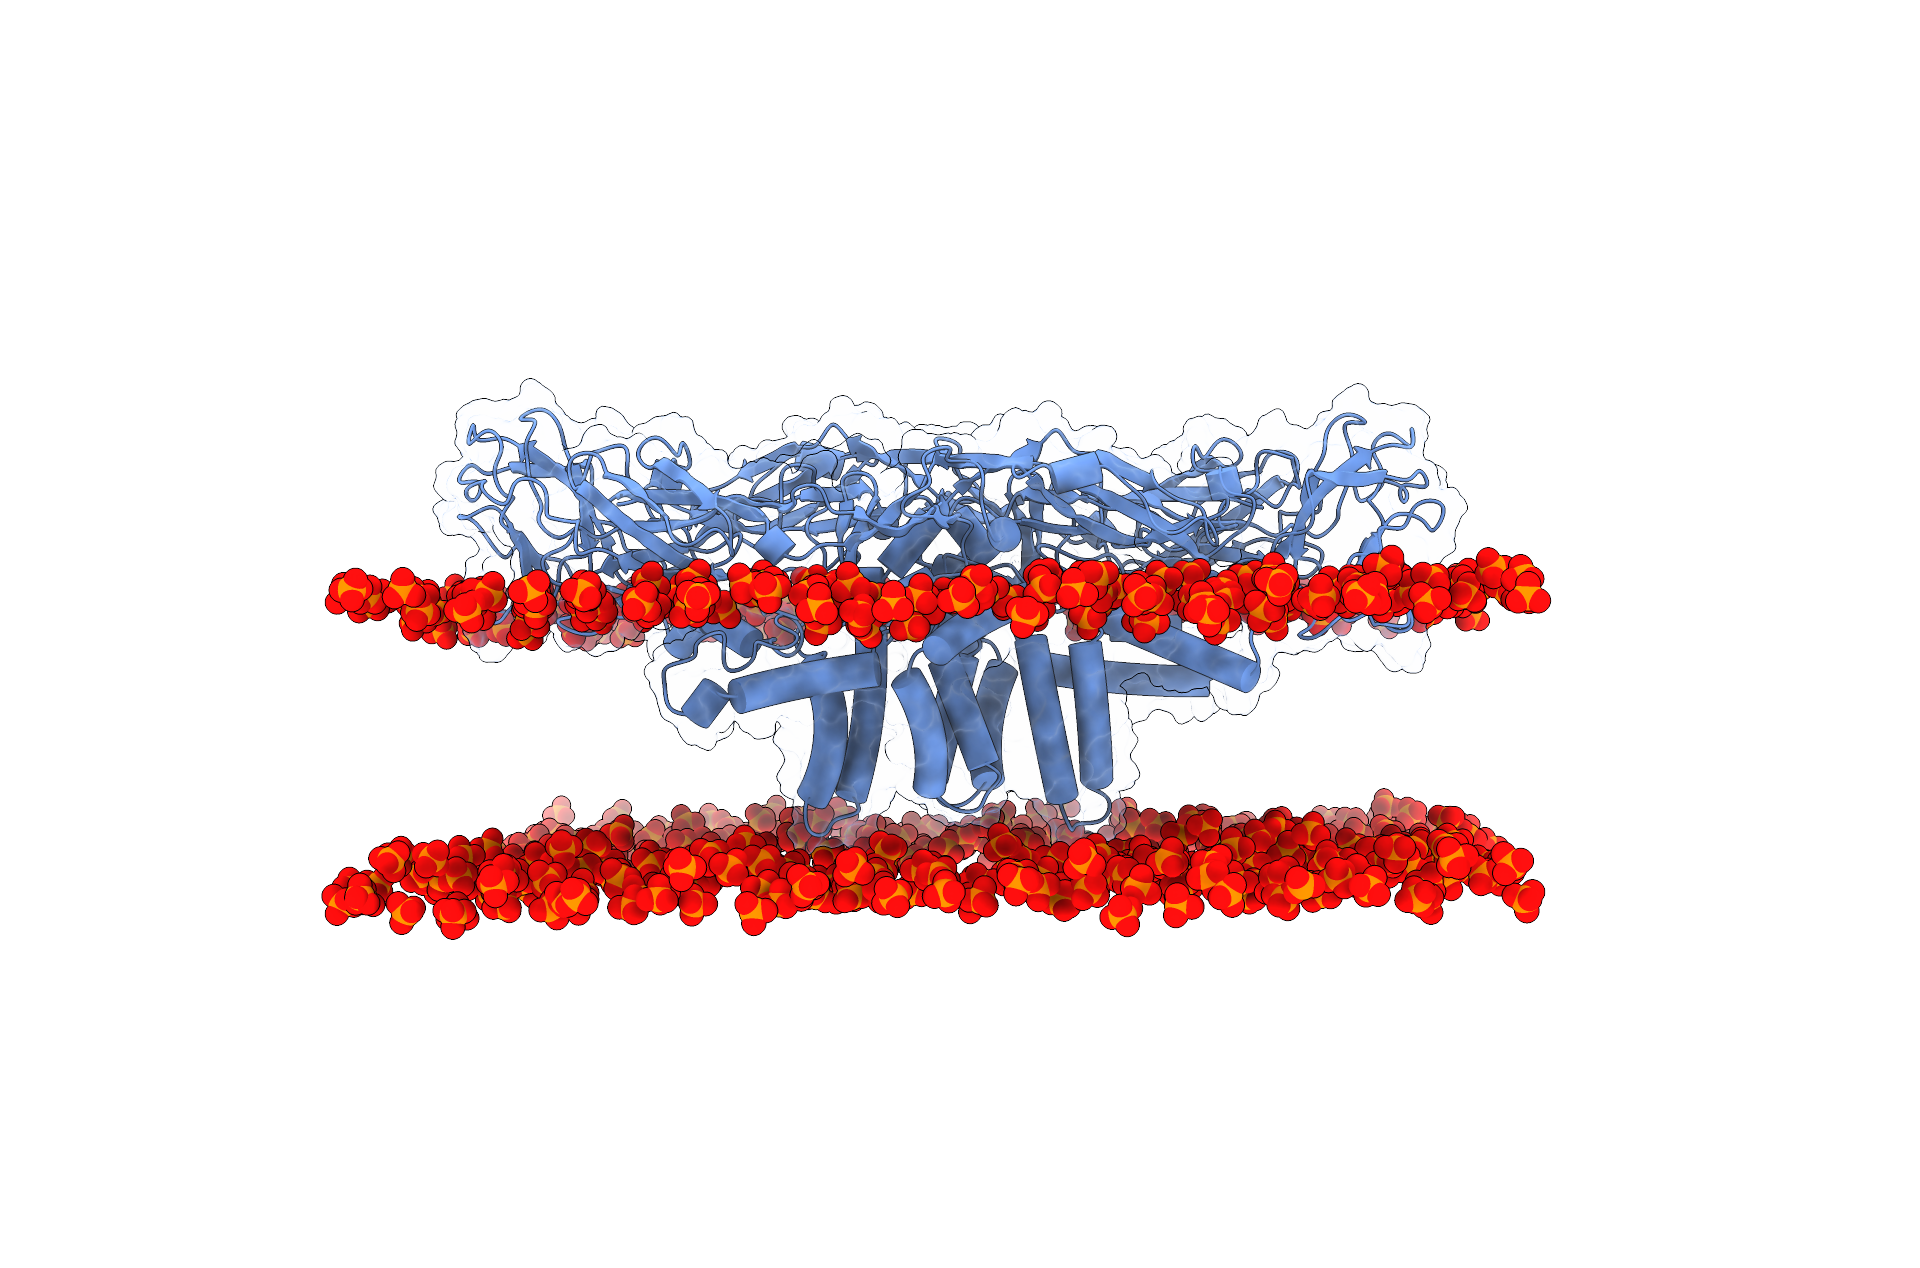
\includegraphics[width=\textwidth]{Figure/denvmem}
 	\caption{Una perra membranota...}
 	\label{fig:enter-label}
 \end{figure}
\section{Section 2}
    \subsection{Subsection 2}

\chapter{Resultados}
\label{ch3}

\section{microemu}
    \subsection{Subsection 1}


	
\section{Section 2}
    \subsection{Subsection 2}

\include{Chapter4}

\chapter{Conclusiones}
\label{ch5}

\section{Section 1}
    \subsection{Subsection 1}
 Como dice este pendejo \cite{Barzon2016,pablin,LeBlanc2012} \ac{DENV} hasupdhgas \ac{DENV}
\section{Section 2}
    \subsection{Subsection 2}


%\bibliographystyle{achemso} 
\bibliography{tesisss}


\appendix

\chapter{Apéndice A}
\label{chap: Appendix A}

% include appendix if any
La presente tesis ha contado con el apoyo de Modelos de Lenguaje de Gran Tamaño (LLM), específicamente \textbf{ChatGPT}, exclusivamente con el propósito de mejorar la redacción y claridad del texto. En ningún caso se utilizó esta herramienta para la obtención, procesamiento, análisis o interpretación de resultados científicos, ni para la generación de contenido académico original.
Todas las imágenes creadas para este documento se realizaron utilizando herramientas de modelado molecular o de creación de imágenes científicas (Inkscape, ChimeraX, VMD, MOE, Biorender, Illustrate)




\end{document}
